This section presents the technical aspects of our implementation. Firstly, we introduce the notation and conventions adopted that are necessary to fully detail the model of our GNSS factor. Later, we briefly introduce ORB-SLAM3 \cite{campos2021orbslam3}, the state-of-the-art framework Visual-Inertial SLAM that we use in our method. We refer the reader to the original ORB-SLAM3 publication for the full details on such framework. Finally, we detail the formulation of our GNSS factor.

\subsection{Notation}
Figure~\ref{fig:frames} shows the coordinate frames used in this work. $\worldCoordSystem$ represents the world frame and $\bodyCoordSystem$ represents the body frame, that we place in the IMU sensor. $\vec{a}^{S}$ represents the coordinates of a geometry entity $\vec{a}$ with respect to the reference frame $S$. $\rotationCoord{\worldCoordSystem}{\bodyCoordSystem} \in SO(3)$ refers to the rotation of $\bodyCoordSystem$ with respect to $\worldCoordSystem$, and $\translationCoord{\worldCoordSystem}{\bodyCoordSystem} \in \mathbb{R}^3$ represents the translation of the reference frame $\bodyCoordSystem$ expressed in the frame $\worldCoordSystem$. The rigid transformation formed by the rotation $\rotationCoord{\worldCoordSystem}{\bodyCoordSystem}$ and the translation $\translationCoord{\worldCoordSystem}{\bodyCoordSystem}$ is denoted as $\rigidTransformCoord{\worldCoordSystem}{\bodyCoordSystem} \in SE(3)$, and transforms points in homogeneous coordinates from the reference frame ${\bodyCoordSystem}$ to the reference frame ${\worldCoordSystem}$. For global positioning measurements, $\translationCoord{\bodyCoordSystem}{\firstGPSCoordSystem} \in \mathbb{R}^3$ is the position of the GNSS antenna in the body frame, and is assumed to be known from a calibration stage. All GNSS measurements are transformed to the local Cartesian frame that we denote as ${\coordIndex{\firstGPSCoordSystem}{0}}$. We detail below how we choose such reference frame.

\begin{figure}[!t]
    \centering
    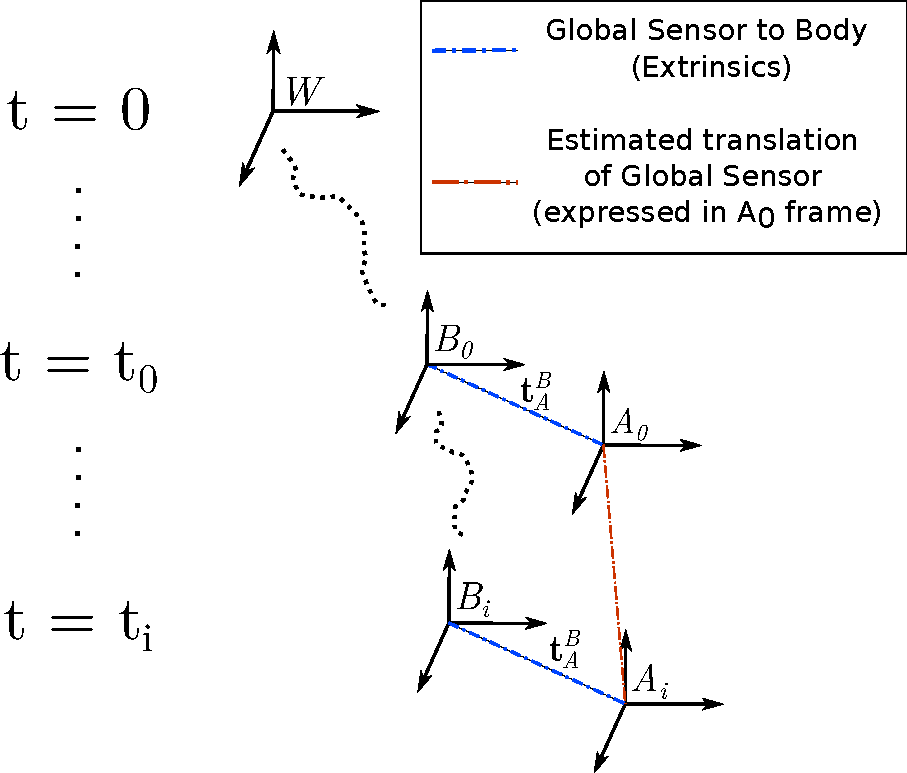
\includegraphics[width=\linewidth]{images/frames.pdf}
    \caption{Reference Frames used in this work. The position of the GNSS antenna in the body frame is represented with a translation and shown with a blue line, and can be obtained from the calibration of the system. The red line represents the estimated translation of the GNSS antenna from time $t_0$ to time $t_i$. This 3D vector is compared with the GNSS measurements in the GNSS error residual $\mathbf{r}_{\mathcal{G}_{i}}$. Both vectors are expressed in ${\coordIndex{\firstGPSCoordSystem}{0}}$ frame.}
    \label{fig:frames}
\end{figure}

\subsection{ORB-SLAM3}
ORB-SLAM3 is a state-of-the-art visual-inertial SLAM framework evolved from ORB-SLAM2 \cite{mur2017orb} and ORB-SLAM-VI \cite{mur2017visual}. With respect to ORB-SLAM-VI, ORB-SLAM3 proposes a substantially more robust inertial initialization based on maximum-a-posteriori estimates. As it is common in current SLAM systems, the processing is split into multiple threads to exploits multi-core architectures. Specifically, ORB-SLAM3 implements a tracking thread, a local mapping thread and a loop closure and map merging thread. The tracking thread estimates the pose of the current frame by minimizing the reprojection error and incorporating IMU constraints into the optimization by pre-integration \cite{forster2017onmanifold}. It also contains the heuristics for deciding whether a frame becomes a keyframe. The mapping thread main task is a visual-inertial bundle adjustment on a sliding window of keyframes, although it also performs auxiliary map management tasks such as point and keyframe culling. Finally, the loop closure and map merging thread ensures the global consistency of large maps by recognizing revisited places and correcting the drift, and joining separate maps if a common overlap is detected.

From the results in \cite{cremona2022evaluation}, ORB-SLAM3 presents an acceptable accuracy in arable lands for short camera trajectories, but long-term navigation is still challenging. The authors propose a novel loop closure algorithm to correct the drift. However, even with such improvement, loop closure keeps being challenging due to the similarity in appearance of the local visual features. As a result, visual SLAM systems may accumulate drift when loop closures are not detected or the estimation may be corrupted by false loop detections.

\subsection{GNSS-Stereo-Inertial Fusion}
In this work, we formulate a tightly-coupled approach for fusing visual, inertial and GNSS data. Firstly, GNSS measurements are associated to the timestamp of a keyframe according to their temporal proximity. If there is a keyframe with a temporal difference under a specific threshold, the GNSS constraint is set to this keyframe. GNSS readings that are not close in time to any keyframe are discarded (see an illustration of this approach in Figure~\ref{fig:association}). While this is an approximation, we found that, given the high variance of conventional GNSS, a sufficiently small threshold and appropriate keyframe management policy makes its effect negligible. 

The first GNSS reading that is associated with a keyframe determines the position of $\coordIndex{\firstGPSCoordSystem}{0}$, the Cartesian frame for our global position measurements (see Figure~\ref{fig:frames}). We choose $\coordIndex{\firstGPSCoordSystem}{0}$ as a East-North-Up (ENU) local Cartesian frame. The subsequent GNSS measurements are transformed to be expressed in $\coordIndex{\firstGPSCoordSystem}{0}$, and we refer to them as $\noisyMeasurement_{i}$, where $t_i$ is the timestamp of the corresponding keyframe. This is done once the IMU is initialized. If the map is reset, the process of selecting $\coordIndex{\firstGPSCoordSystem}{0}$ is repeated. 

\begin{figure}[!t]
    \centering
    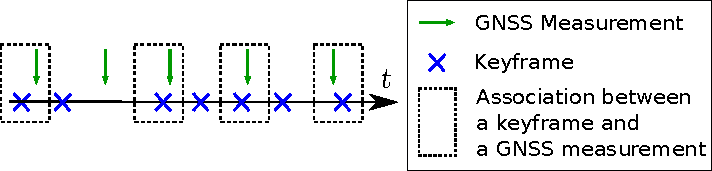
\includegraphics[width=\linewidth]{images/association.pdf}
    \caption{Temporal association between keyframes and GNSS measurements. %Keyframes are depicted with blue crosses on the temporal line and GNSS measurements are depicted with green arrows. 
    GNSS measurements are discarded if they are further than specific temporal threshold from any keyframe.}
    \label{fig:association}
\end{figure}

Our GNSS-Stereo-Inertial fusion is done in the local bundle adjustment of a sliding window of keyframes and 3D points observed from them. Figure~\ref{fig:graph} shows the factor graph corresponding to such optimization. The state variables to optimize are $\mathcal{X} = \{\mathcal{X}_{B}, \mathcal{L}\}$, where $\mathcal{X}_{B} = [\systemState_{1},\dots,\systemState_{i},\dots,\systemState_{N}]$ is the set of sensor states for a window covering the last $N$ keyframes and $\mathcal{L}= [\mathbf{y}_{1},\dots,\mathbf{y}_{j},\dots,\mathbf{y}_{M}]$ is the set of landmarks states that were measured during those last $N$ keyframes. The sensor state $\systemState_{i}$ at the time instant $i$ is
%
\begin{equation}
    \systemState_{i} = [\rigidTransformCoord{\worldCoordSystem}{\coordIndex{\bodyCoordSystem}{i}}, \coordIndex{\linearVelocity}{i}^\top, \bias_{a_i}^\top, \bias_{g_i}^\top],
\end{equation}
%
which contains the sensor rigid transformation with respect to the world frame $\rigidTransformCoord{\worldCoordSystem}{\coordIndex{\bodyCoordSystem}{i}} \in SO(3)$, its local velocity $\coordIndex{\linearVelocity}{i} \in \mathbb{R}^3$ and the accelerometer and gyroscope bias $\bias_{a_i} \in \mathbb{R}^3$ and $\bias_{g_i} \in \mathbb{R}^3$. Landmarks are represented by their Euclidean coordinates in the world frame, i.e., $\mathbf{y}_{j} = [X^W, Y^W, Z^W]^\top \in \mathbb{R}^3$

In comparison to ORB-SLAM3, a GNSS error term is added to the cost function. Note that, as shown in Figure~\ref{fig:association}, some keyframes may not have an associated GNSS measurement. %Then the cost function to be minimized results in:
Then, our GNSS-Stereo-Inertial mapping optimization can be stated as follows
%
\begin{equation}
\begin{split}
    \hat{\mathcal{X}} = \argmin_{\mathcal{X}} \left( \sum_{i=1}^N \lVert \mathbf{r}_{\mathcal{I}_{i-1,i}}  \rVert^2_{\Sigma_{\mathcal{I}_{i-1,i}}^{-1}} +\right. \\ 
    \left. + \sum_{j=1}^M \sum_{i \in \mathcal{K}_j} \rho \left( \lVert \mathbf{r}_{\mathcal{V}_{ij}} \rVert_{\Sigma_{{V}_{ij}}^{-1}} +\right) \right. \\
    \left. + \sum_{i \in \mathcal{N}^*} \rho \left( \lVert \mathbf{r}_{\mathcal{G}_{i}} \rVert_{\Sigma_{\mathcal{G}_{i}}^{-1}} +\right) \right),
\end{split}
\end{equation}
%
where $\mathcal{N}^*$ is the set of keyframes that have an associated GNSS measurement. The three addends correspond, respectively, to the inertial, visual and GNSS constraints. For completitude we will detail the three of them, although the first two are used exactly as proposed in ORB-SLAM3 and the third one is our novel contribution.

The inertial residual is defined as follows
%
\begin{equation}
\mathbf{r}_{\mathcal{I}_{i-1,i}} = [\mathbf{r}_{\Delta \mathbf{R}_{i-1,i}}^\top, \mathbf{r}_{\Delta \mathbf{v}_{i-1,i}}^\top, \mathbf{r}_{\Delta \mathbf{p}_{i-1,i}}^\top]^{\top},
\end{equation}
%
where $\mathbf{r}_{\Delta \mathbf{R}_{i-1,i}}$, $\mathbf{r}_{\Delta \mathbf{v}_{i-1,i}}$ and $\mathbf{r}_{\Delta \mathbf{p}_{i-1,i}}$ correspond to orientation, velocity and position residuals that have the following form
%
\begin{equation}
\footnotesize
\begin{aligned}
\mathbf{r}_{\Delta \mathbf{R}_{i-1,i}} &= \log \left( \Delta \mathbf{R}_{i-1,i}^\top \mathbf{R}_{i-1}^\top \mathbf{R}_{i} \right) \\
\mathbf{r}_{\Delta \mathbf{v}_{i-1,i}} &= \mathbf{R}_{i}^\top \left( \mathbf{v}_{i} - \mathbf{v}_{i-1} - \mathbf{g}\Delta t_{i-1,i} \right) - \Delta \mathbf{v}_{i-1,i} \\
\mathbf{r}_{\Delta \mathbf{p}_{i-1,i}} &= \mathbf{R}_{i}^\top \left( \mathbf{p}_{i} - \mathbf{p}_{i-1} - \mathbf{v}_{i} \Delta t_{i-1,i} - \frac{1}{2}\mathbf{g}\Delta t_{i-1,i}^2 \right) - \\ & \ \ \ - \Delta \mathbf{p}_{i-1,i}.
\end{aligned}
\end{equation}
%
The terms denoted as $\Delta \mathbf{R}_{i-1,i}$, $\Delta \mathbf{v}_{i-1,i}$ and $\Delta \mathbf{p}_{i-1,i} $ come from the preintegration of the IMU readings between the time instants $i-1$ and $i$, and are computed together with their on-manifold covariance $\Sigma_{\mathcal{I}_{i-1,i}}$ according to \cite{forster2017onmanifold}. $\mathbf{g}$ stands for the gravity direction, which is set at the system bootstrapping.

The visual residual $\mathbf{r}_{\Delta \mathbf{v}_{i-1,i}}$ is
%
\begin{equation}
    \mathbf{r}_{\mathcal{V}_{ij}} = \mathbf{u}_{ij} - \pi\left( \rigidTransformCoord{C}{\bodyCoordSystem} \rigidTransformCoord{\worldCoordSystem-1}{\bodyCoordSystem} \tilde{\mathbf{y}}_{j} \right),
\end{equation}
%
where $ \tilde{\mathbf{y}}_{j}$ stands for the homogeneous representation of the $j^{th}$ landmark, $\pi(\cdot)$ for the pinhole projection model of a 3D point in homogeneous coordinates in a stereo image, and $\mathbf{u}_{ij}$ the measured image coordinates of the $j^{th}$ landmark in the $i^{th}$ stereo keyframe. The visual covariance of image landmarks $\Sigma_{\mathcal{V}_{ij}}$ is set to the standard 1-pixel standard deviation isotropic Gaussian.

Finally, the GNSS error residual is
%
\begin{equation}
\footnotesize
\mathbf{r}_{\mathcal{G}_{i}} = \noisyMeasurement_{i} -  \rotationCoord{\coordIndex{\firstGPSCoordSystem}{0}}{\worldCoordSystem}\left(\rotationCoord{\worldCoordSystem}{\coordIndex{\bodyCoordSystem}{i}}\translationCoord{\bodyCoordSystem}{\firstGPSCoordSystem} + \translationCoord{\worldCoordSystem}{\coordIndex{\bodyCoordSystem}{i}} - \left(\rotationCoord{\worldCoordSystem}{\coordIndex{\bodyCoordSystem}{0}}\translationCoord{\bodyCoordSystem}{\firstGPSCoordSystem} + \translationCoord{\worldCoordSystem}{\coordIndex{\bodyCoordSystem}{0}} \right)\right).
\end{equation}
%
The second term represents the translation vector of the global sensor (in this case, the GNSS antenna) at time instant $i$ in the reference frame $\coordIndex{\firstGPSCoordSystem}{0}$, as can be seen in Figure~\ref{fig:frames}. $\rotationCoord{\worldCoordSystem}{\coordIndex{\bodyCoordSystem}{0}}$ and $\translationCoord{\worldCoordSystem}{\coordIndex{\bodyCoordSystem}{0}}$, which are the relative rotation and translation between the body and the world frame at time $t_0$, are kept constant during the optimization. $\rotationCoord{\coordIndex{\firstGPSCoordSystem}{0}}{\worldCoordSystem}$ is computed by aligning  the first 20 GNSS measurements  with the poses estimated by ORB-SLAM3 in the same time period using Umeyama's method \cite{umeyama1991least}. After estimating this rotation, it is kept fixed during the whole optimization process. The covariance matrix $\Sigma_{\mathcal{G}_{i}}$ is set from the specifications sheet of our GNSS device in each Cartesian axis
%
\begin{equation}
\Sigma_{\mathcal{G}_{i}} = \begin{bmatrix}
\sigma_x^{2} & 0 & 0\\
0 & \sigma_y^{2} & 0 \\
0 & 0 & \sigma_z^{2}
\end{bmatrix}.
\end{equation}
%
This covariance matrix is defined relative to a tangential plane through the GNSS reported position. The values are expressed in ENU frame. Finally, the Jacobian with respect to the pose error state is defined as
%
\begin{equation}
\frac{\partial \mathbf{r}_{\mathcal{G}_{i}}}{\partial \delta \rigidTransformCoord{\worldCoordSystem}{\coordIndex{\bodyCoordSystem}{i}}} = \left[ \rotationCoord{\coordIndex{\firstGPSCoordSystem}{0}}{\worldCoordSystem}  \rotationCoord{\worldCoordSystem}{\coordIndex{\bodyCoordSystem}{i}} \left[ \translationCoord{\bodyCoordSystem}{\firstGPSCoordSystem}\right]^{\times} \quad -\rotationCoord{\coordIndex{\firstGPSCoordSystem}{0}}{\worldCoordSystem}  \right],
\end{equation}

where $\delta$ indicates that the derivative is computed with respect to a right perturbation in the pose.

%
\begin{figure}[!tb]
    \centering
    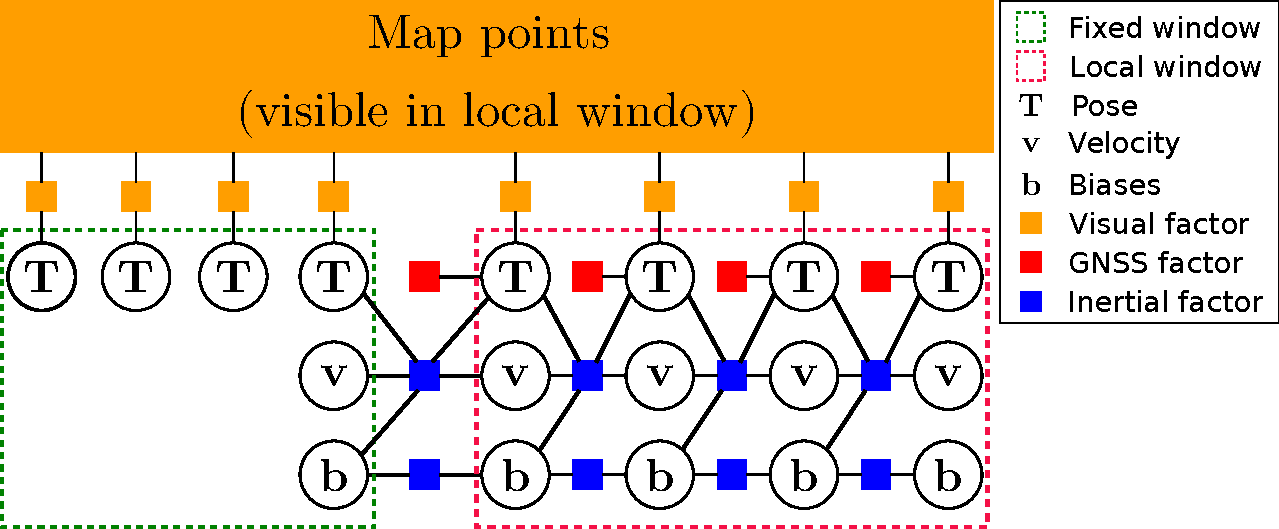
\includegraphics[width=\columnwidth]{images/graph.pdf}
    \caption{Factor Graph corresponding to the Local Bundle Adjustment of our GNSS-Stereo-Inertial SLAM. In comparison to ORB-SLAM3, a GNSS factor (in red) is added to the cost function. The Local Window is composed by the $N$ last keyframes.}
    \label{fig:graph}
\end{figure}
